\begin{intersong}
    \newpage\null
    \begin{center}
        \songsection{Anschlagmuster Gitarre}
    \end{center}
    Hier finden sich drei Basis-Anschlagmuster mit denen sich viele Lieder spielen lassen. Diese sind aus dem \textit{Codex Patomomomensis} kopiert und nach Fußballern benannt. Unter den Liedern sind diese Anschlagmuster teilweise mit ihrem Kürzel angegeben. Ein Pfeil nach unten ist ein Abschlag, ein Pfeil nach oben ein Aufschlag. Ein waagerechter Strich bedeutet, dass der Schlag lang ist. \\
    
    \noindent\textbf{1. Ulf Kirsten (UK)} \newline
    Takt: 2/4, passt aber auch zu 4/4. Rythmus: lang-kurz-kurz.
    \begin{center}
        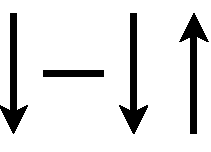
\includegraphics[height=1cm]{Schm-UK.pdf}
    \end{center}
    
    \noindent\textbf{2. Franz Beckenbauer (FB)} \newline
    Takt: 3/4, passt aber auch zu 6/8. Rythmus: lang-kurz-kurz-kurz-kurz.
    \begin{center}
        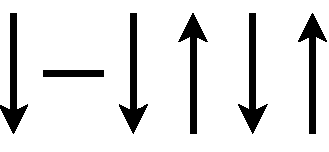
\includegraphics[height=1cm]{Schm-FB.pdf}
    \end{center}
    
    \noindent\textbf{3. Michael Rummenigge (MR)} \newline
    Takt: 4/4. Rythmus: lang-kurz-kurz-kurz-kurz-kurz-kurz.
    \begin{center}
        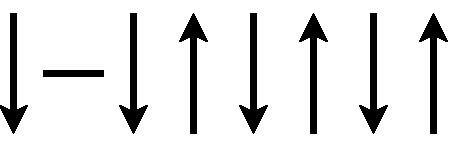
\includegraphics[height=1cm]{Schm-MR.pdf}
    \end{center}
    

\end{intersong}